%%%%%%%%%%%%%%%%%%%%%%%%%%%%%%%%%%%%%%%%%
% Beamer Poster Template
% Original template from C. Lazaris
% Modified by Stephen Kelly
% LaTeX Template
%
%%%%%%%%%%%%%%%%%%%%%%%%%%%%%%%%%%%%%%%%%

%----------------------------------------------------------------------------------------
%	PACKAGES AND OTHER DOCUMENT CONFIGURATIONS
%----------------------------------------------------------------------------------------

\documentclass[final]{beamer}
\listfiles % record the packages used at the end of the .log file upon compilation
\usepackage[scale=1.24]{beamerposter} % Use the beamerposter package for laying out the poster
\usepackage{hyperref}
\usepackage{tikz}                     % This is to add logo
\usepackage{tikzpagenodes}            % Finer tuning

\usetheme{confposter} % Use the confposter theme supplied with this template

\setbeamercolor{block title}{fg=dblue!70,bg=white} % Colors of the block titles
\setbeamercolor{block body}{fg=black,bg=white} % Colors of the body of blocks
\setbeamercolor{block alerted title}{fg=white,bg=dblue!70} % Colors of the highlighted block titles
\setbeamercolor{block alerted body}{fg=black,bg=dblue!10} % Colors of the body of highlighted blocks
% Many more colors are available for use in beamerthemeconfposter.sty
\usepackage{graphicx} % need these two for the frames aroundthe figures
\usepackage[export]{adjustbox}
%-----------------------------------------------------------
% Define the column widths and overall poster size
% To set effective sepwid, onecolwid and twocolwid values, first choose how many columns you want and how much separation you want between columns
% In this template, the separation width chosen is 0.024 of the paper width and a 4-column layout
% onecolwid should therefore be (1-(# of columns+1)*sepwid)/# of columns e.g. (1-(4+1)*0.024)/4 = 0.22
% Set twocolwid to be (2*onecolwid)+sepwid = 0.464
% Set threecolwid to be (3*onecolwid)+2*sepwid = 0.708

\newlength{\sepwid}
\newlength{\onecolwid}
\newlength{\twocolwid}
\newlength{\threecolwid}
\setlength{\paperwidth}{48in} % A0 width: 46.8in
\setlength{\paperheight}{36in} % A0 height: 33.1in
\setlength{\sepwid}{0.024\paperwidth} % Separation width (white space) between columns
\setlength{\onecolwid}{0.22\paperwidth} % Width of one column
\setlength{\twocolwid}{0.464\paperwidth} % Width of two columns
\setlength{\threecolwid}{0.708\paperwidth} % Width of three columns
\setlength{\topmargin}{0.5in} % Reduce the top margin size
%-----------------------------------------------------------

\usepackage{graphicx}  % Required for including images

\usepackage{booktabs}  % Top and bottom rules for tables

%\usepackage{helvet}    % Use Helvetica
%\renewcommand{\familydefault}{\sfdefault}

%----------------------------------------------------------------------------------------
%	TITLE SECTION 
%----------------------------------------------------------------------------------------

\title{\LARGE{Automated ChIP-Seq Analysis and Reporting Pipeline}} % Poster title

\author{Stephen Kelly\textsuperscript{1,2}, Igor Dolgalev\textsuperscript{1-5}, Charalampos Lazaris\textsuperscript{3-5} \& Aristotelis Tsirigos\textsuperscript{1-5}} % Author(s)

\institute{
\normalsize{
~\textsuperscript{1}Applied Bioinformatics Center \&~\textsuperscript{2}Genome Technology Center, NYU School of Medicine, NY 10016, USA,
~\textsuperscript{3}Department of Pathology,
~\textsuperscript{4}NYU Cancer Institute and Helen L. and Martin S. Kimmel Center for Stem Cell Biology,
~\textsuperscript{5}Center for Health Informatics \& Bioinformatics,
}
} % Institution(s)



%----------------------------------------------------------------------------------------

\begin{document}

\addtobeamertemplate{headline}{} 
{\begin{tikzpicture}[remember picture, overlay]
      \node [anchor=north west]  at ([xshift=10.5cm,yshift=-3.5cm]current page.north west)
      {
\includegraphics[height=5cm]{./Figures/NYULMC_white}};
 \end{tikzpicture}} % Add logo

% \addtobeamertemplate{block end}{}{\vspace*{1ex}} % White space under blocks
% \addtobeamertemplate{block alerted end}{}{\vspace*{1ex}} % White space under highlighted (alert) blocks
% \addtobeamertemplate{beamerboxesrounded end}{}{\vspace*{2ex}} % White space under blocks
% ^ this doesn't work.. 
\setlength{\belowcaptionskip}{0.01ex} % White space under figures % previously 0.5 for both of these
% \setlength\belowdisplayshortskip{0.1ex} % White space under equations

\begin{frame}[t] % The whole poster is enclosed in one beamer frame
% FRAME % ~~~~~~~~~~~~~~~~~~~~~~~~~~~~~~ % ~~~~~~~~~~~~~~~~~~~~~~~~~~~
% ~~~~~~~~~~~~~~~~~~~~~~~~~~~~~~~~~~~~~~ % ~~~~~~~~~~~~~~~~~~~~~~~~~~~

\begin{columns}[t] % The whole poster consists of three major columns, the second of which is split into two columns twice - the [t] option aligns each column's content to the top

\begin{column}{\sepwid}\end{column} % Empty spacer column

\begin{column}{\onecolwid} % The first column
% 1 % ~~~~~~~~~~~~~~~~~~~~~~~~~~~~~~ % ~~~~~~~~~~~~~~~~~~~~~~~~~~~

%----------------------------------------------------------------------------------------
%	OBJECTIVES
%----------------------------------------------------------------------------------------

\begin{beamerboxesrounded}{Objective}

Develop a reproducible ChIP-Seq pipeline that can adapt to varying numbers of samples, treatment groups, and parameter sets while allowing for user expansion with custom programs and analysis tasks. 

\end{beamerboxesrounded}\hfill

%----------------------------------------------------------------------------------------
%	
%----------------------------------------------------------------------------------------


\begin{beamerboxesrounded}{Pipeline usage summary}


\begin{enumerate}
\item Create new directory for analysis from a clone of the pipeline repository (Figure~\ref{fig:github_repo})
\item Set input files (fastq, bam)
\item Generate sample sheet with pipeline-provided scripts
\item (Optional) Modify parameters as needed, add custom tasks
\item Run pipeline
\item Compile automatic report
\end{enumerate}

\begin{figure}
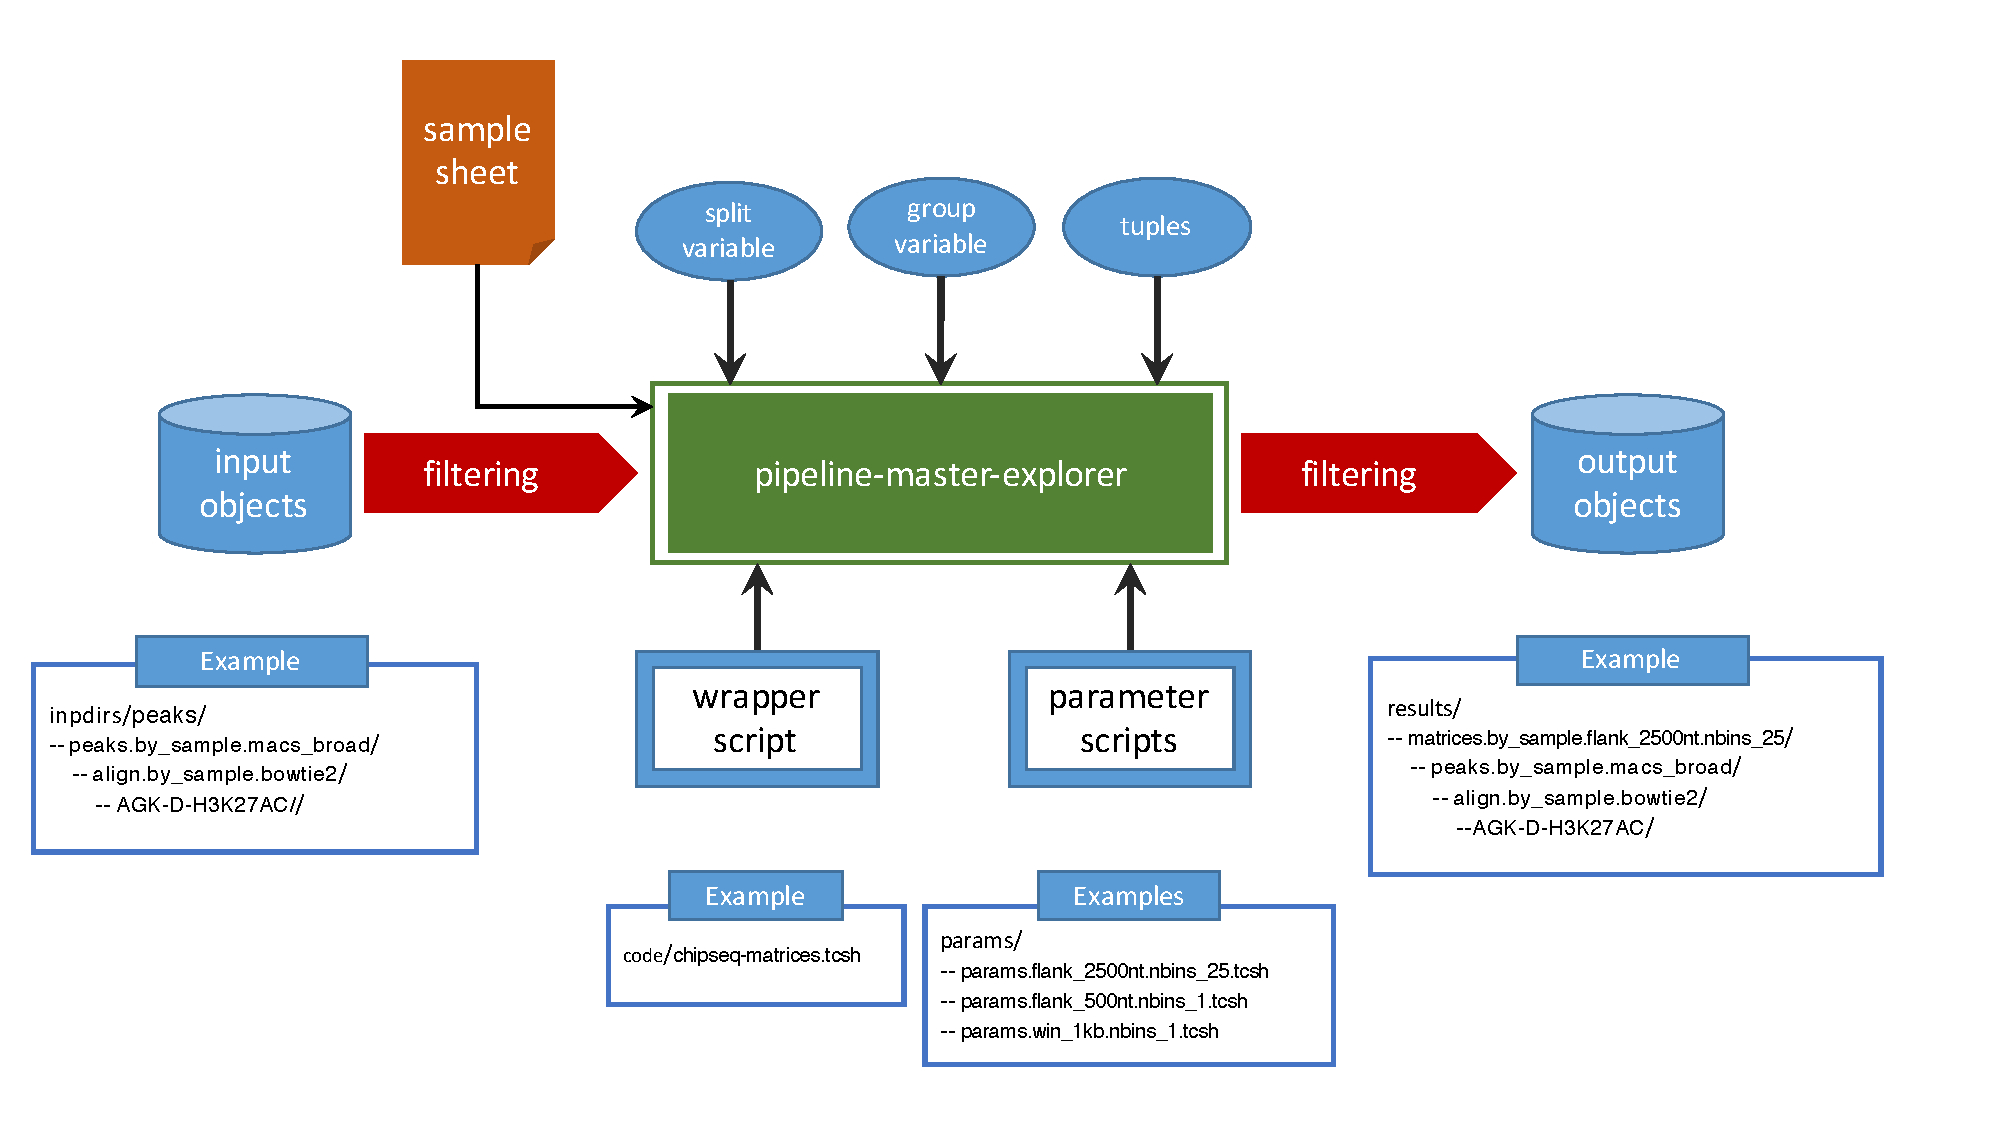
\includegraphics[width=1.0\linewidth]{./Figures/ChIPSeq_flowchart}
\caption{ChIP-Seq pipeline programmatic workflow. All sets of parameters are evaluated for each pipeline task in a combinatorial fashion}
\label{fig:flowchart}
\end{figure}
 % (Table~\ref{tab:toolkit}).
\end{beamerboxesrounded}\hfill

\begin{table}
\centering
\resizebox{\columnwidth}{!}{%
\begin{tabular}{l l}
\toprule
\textbf{ChIP-Seq Pipeline tasks} & \textbf{Programs Used}\\
\midrule
Alignment             &  bowtie2\\
Alignment Stats             &  bowtie2, \textbf{R}\\
Quality Control &  FastQC, deepTools\\
Peak Calling     &  MACS\\
Matrix Correlation    &  \textbf{GenomicTools}\\ 
Principal Component Analysis      &  \textbf{R}\\
Heatmap Clustering        &  \textbf{R}\\
Differential Peak Binding          &  DiffBind\\ 
Visualization         &  \textbf{R}\\
Automatic Reporting   & \textbf{R, \LaTeXe~} \\ %  \fmtversion
\bottomrule
\end{tabular}%
}
\caption{ChIP-Seq pipeline standard components. Internally developed methods listed in bold.}
\label{tab:toolkit}
\end{table}


% 1 % ~~~~~~~~~~~~~~~~~~~~~~~~~~~~~~ % ~~~~~~~~~~~~~~~~~~~~~~~~~~~
\end{column} % End of the first column

\begin{column}{\sepwid}\end{column} % Empty spacer column

\begin{column}{\twocolwid} % Begin a column which is two columns wide (column 2)
% 2 % ~~~~~~~~~~~~~~~~~~~~~~~~~~~~~~ % ~~~~~~~~~~~~~~~~~~~~~~~~~~~

\begin{columns}[t,totalwidth=\twocolwid] % Split up the two columns wide column
% 2.0 % ~~~~~~~~~~~~~~~~~~~~~~~~~~~~~~ % ~~~~~~~~~~~~~~~~~~~~~~~~~~~

% make this a single double wide column
\begin{column}{\onecolwid}%\vspace{-.6in} % The first column within column 2 (column 2.1) 
% 2.1 % ~~~~~~~~~~~~~~~~~~~~~~~~~~~~~~ % ~~~~~~~~~~~~~~~~~~~~~~~~~~~

%----------------------------------------------------------------------------------------
%	
%----------------------------------------------------------------------------------------
\begin{beamerboxesrounded}{} % Auto-report Sample Output

% ChIP-Seq report snapshots go here, double wide!
\begin{figure}
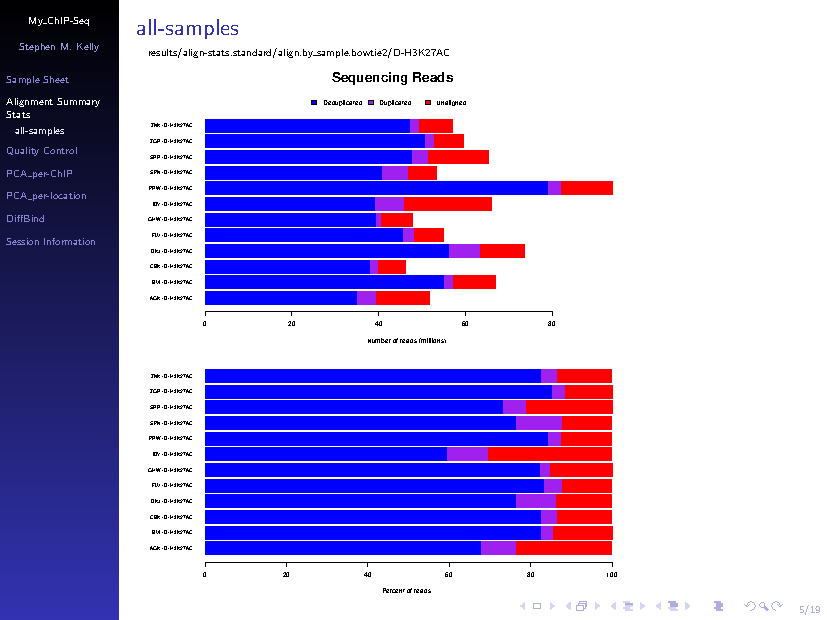
\includegraphics[width=1.0\linewidth, frame]{./Figures/alignStats}
\caption{Alignment summary statistics}
\label{fig:alignStats}
\end{figure}

% \vspace{10cm}

\begin{figure} % fastqc
% 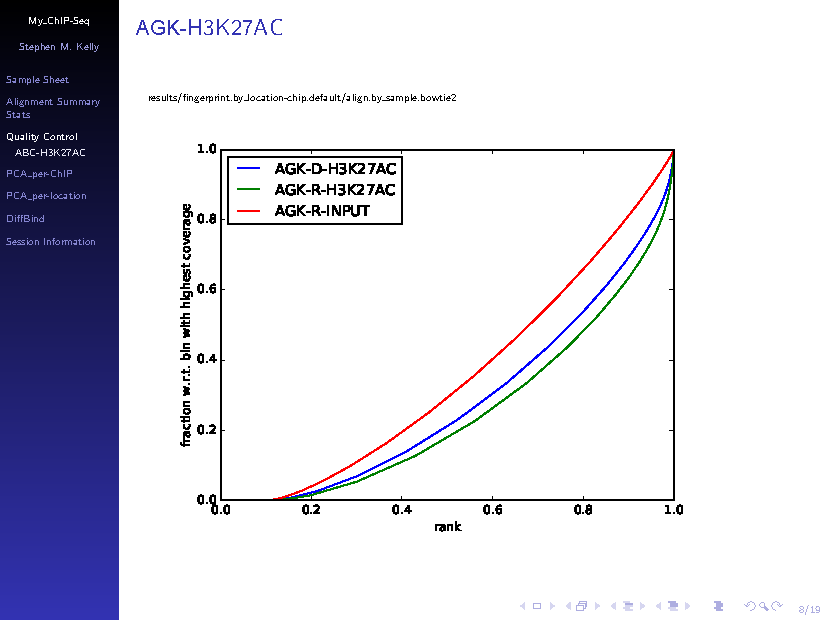
\includegraphics[width=1.0\linewidth, frame]{./Figures/fingerprint}
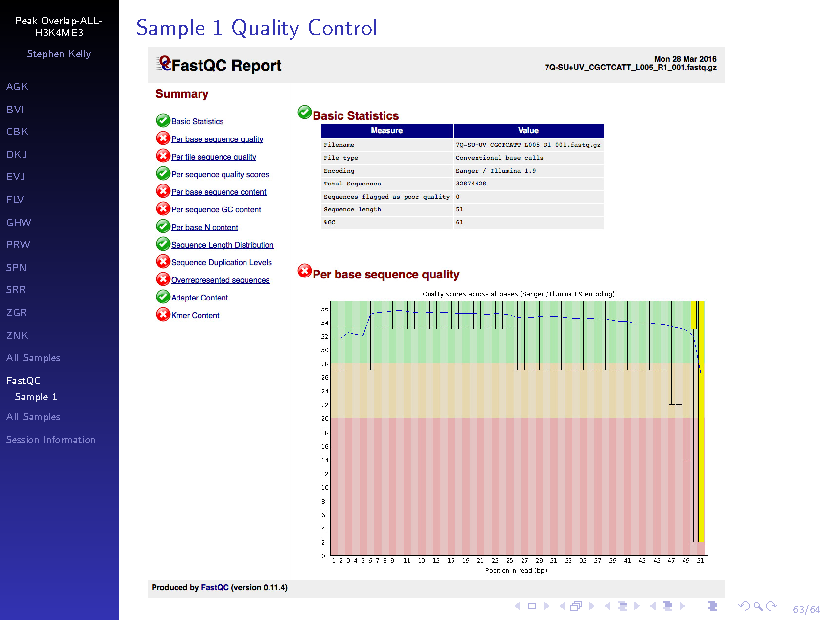
\includegraphics[width=1.0\linewidth, frame]{./Figures/fastqc_report}
\caption{Quality control metrics}
\label{fig:fingerprint}
\end{figure}


\begin{figure}
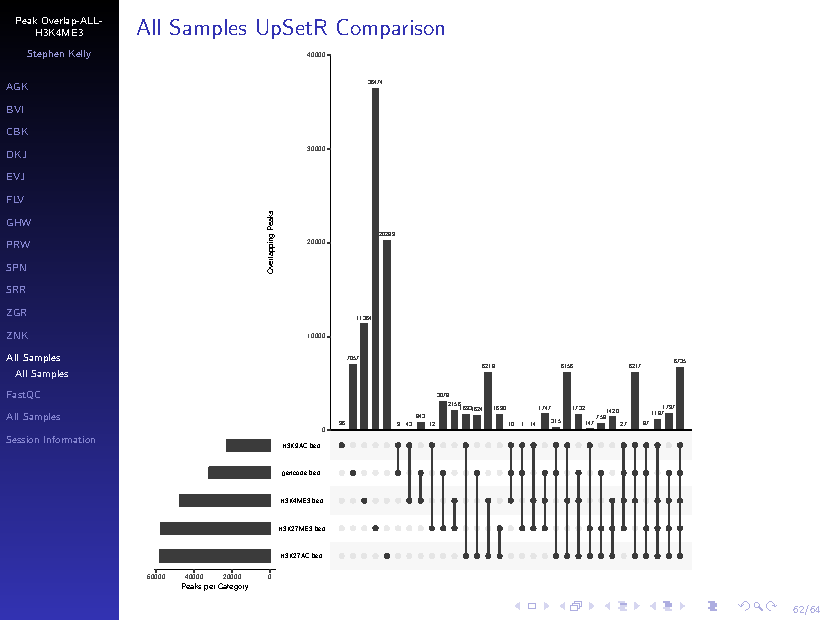
\includegraphics[width=1.0\linewidth, frame]{./Figures/peaks_UpSetR}
\caption{Peak overlap UpSet plot}
\label{fig:five_way_venn}
\end{figure}


\end{beamerboxesrounded}\hfill


% 2.1 % ~~~~~~~~~~~~~~~~~~~~~~~~~~~~~~ % ~~~~~~~~~~~~~~~~~~~~~~~~~~~
\end{column} % End of column 2.1

\begin{column}{\onecolwid}% The second column within column 2 (column 2.2)
% 2.2 % ~~~~~~~~~~~~~~~~~~~~~~~~~~~~~~ % ~~~~~~~~~~~~~~~~~~~~~~~~~~~

%----------------------------------------------------------------------------------------
%	
%----------------------------------------------------------------------------------------

\begin{beamerboxesrounded}{}% \phantom{Auto-report Output}


% \begin{minipage}{\linewidth} % I tried using a minipage here but didn't like it
\begin{figure}
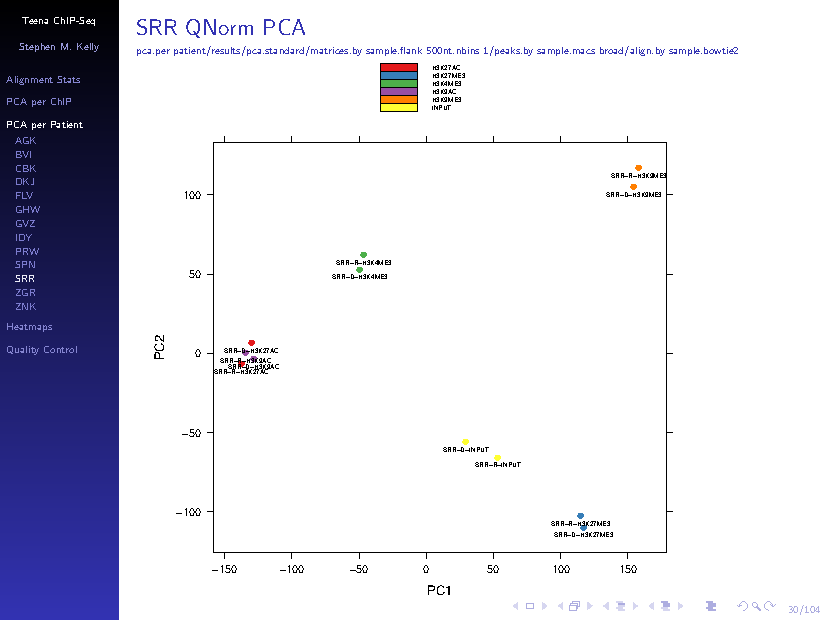
\includegraphics[width=1.0\linewidth, frame]{./Figures/PCA_report}
\caption{Principal component analysis}

\label{fig:PCA}
\end{figure}
% \end{minipage}

% \vspace{10cm}

% \vfill
% \bigskip
% \bigskip
% \bigskip

% \begin{minipage}{\linewidth}

\begin{figure}
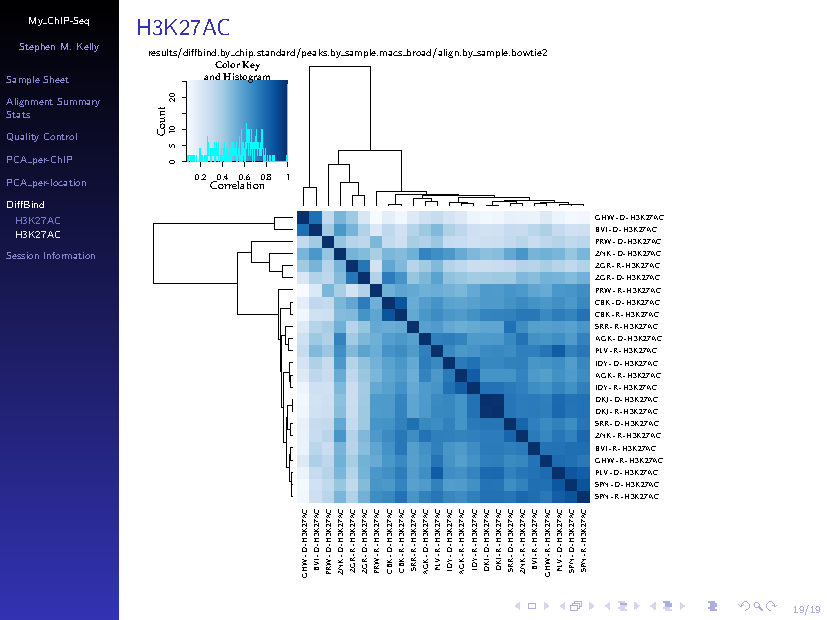
\includegraphics[width=1.0\linewidth, frame]{./Figures/heatmap}
\caption{Differential binding heatmaps}
\label{fig:heatmap}
\end{figure}

\begin{figure}
% 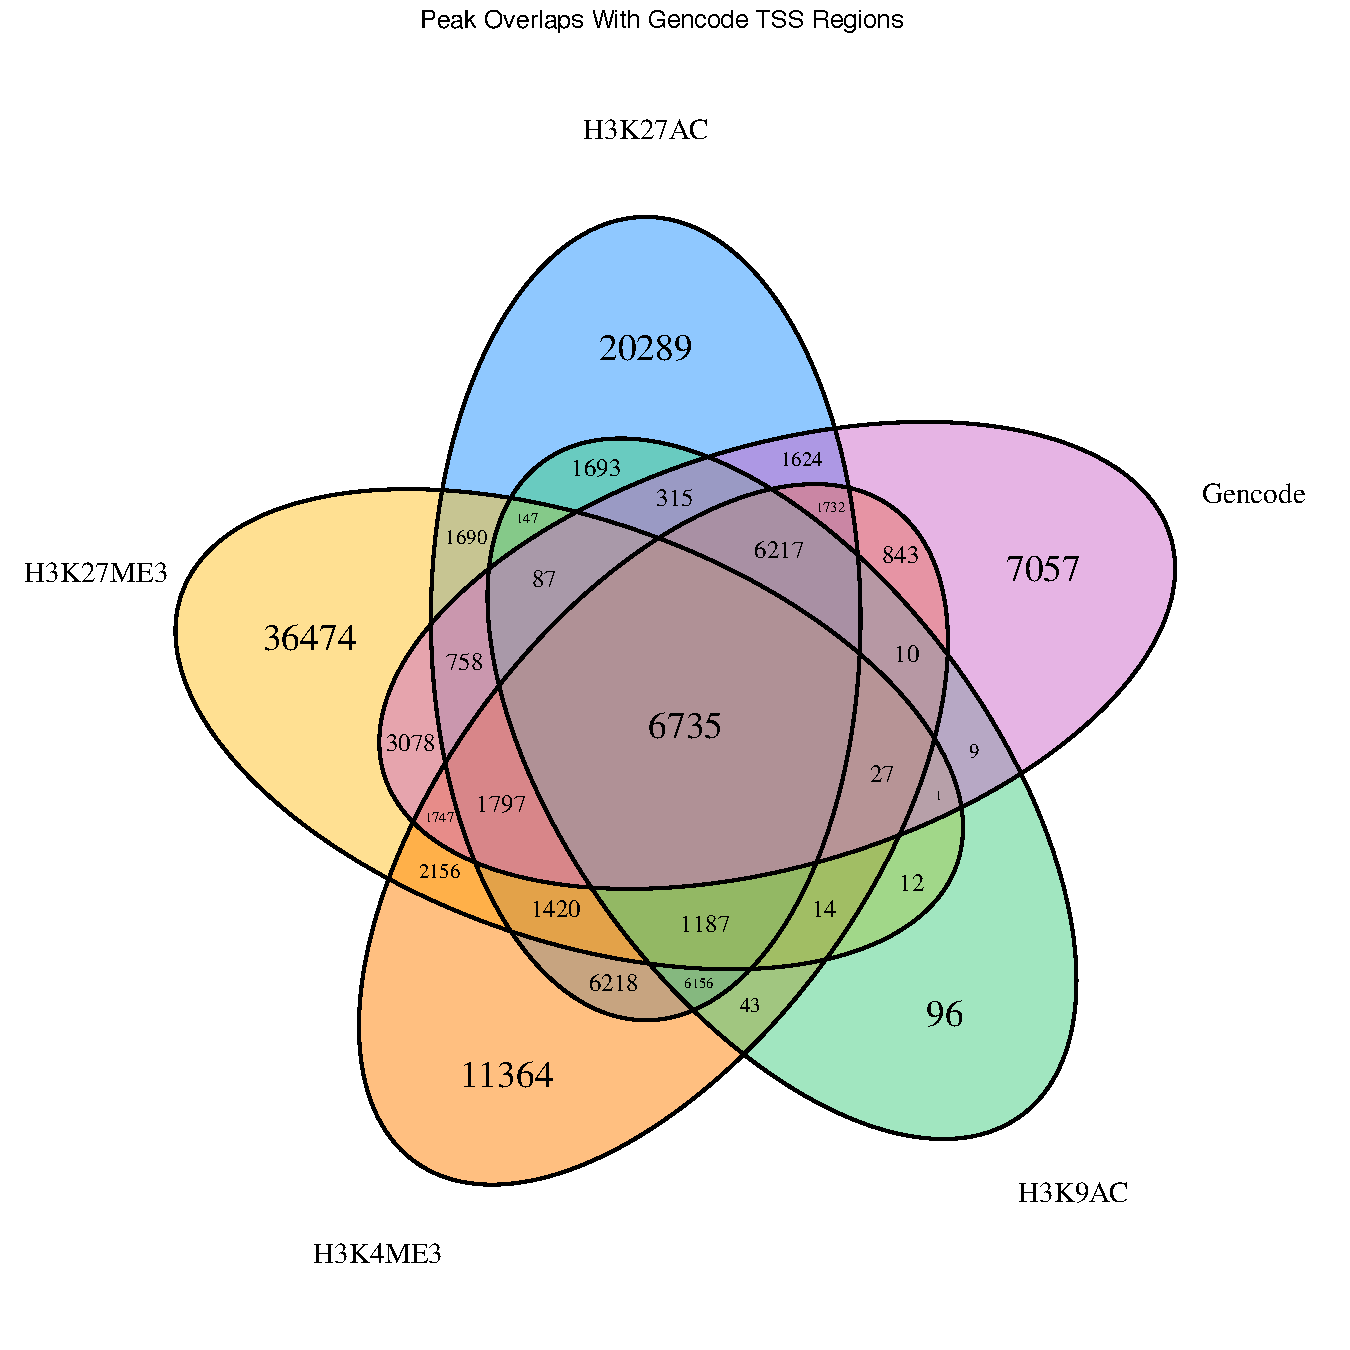
\includegraphics[width=0.7\linewidth, frame]{./Figures/fiveway-venn}
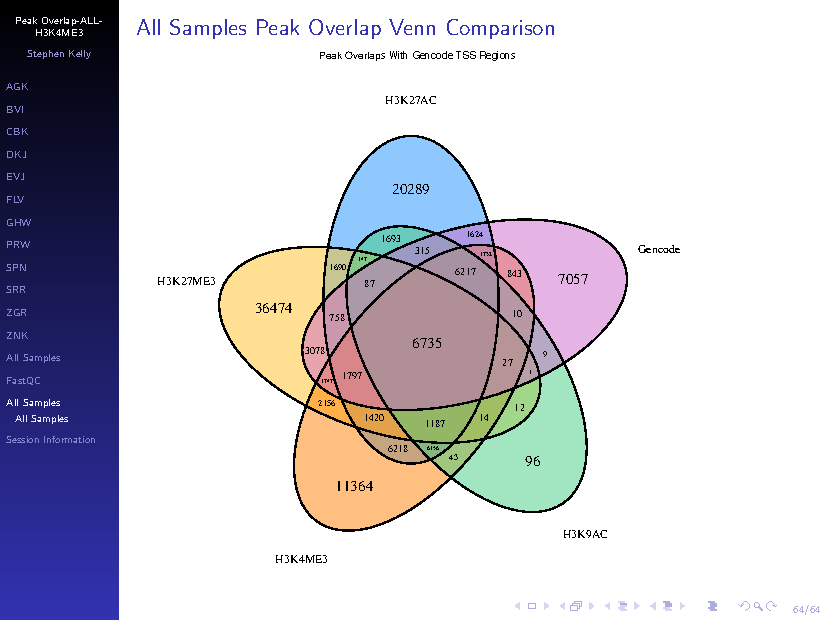
\includegraphics[width=1.0\linewidth, frame]{./Figures/fiveway-venn_report}
\caption{Peak overlap venn diagram}
\label{fig:five_way_venn}
\end{figure}

% \end{minipage}


\end{beamerboxesrounded}\hfill

% 2.2 % ~~~~~~~~~~~~~~~~~~~~~~~~~~~~~~ % ~~~~~~~~~~~~~~~~~~~~~~~~~~~
\end{column} % End of column 2.2

% 2.0 % ~~~~~~~~~~~~~~~~~~~~~~~~~~~~~~ % ~~~~~~~~~~~~~~~~~~~~~~~~~~~
\end{columns} % End of the split of column 2 - any content after this will now take up 2 columns width


\begin{columns}[t,totalwidth=\twocolwid] % Split up the two columns wide column again
% 2.? % ~~~~~~~~~~~~~~~~~~~~~~~~~~~~~~ % ~~~~~~~~~~~~~~~~~~~~~~~~~~~

% \begin{column}{\onecolwid} % The first column within column 2 (column 2.1)
% % 2.?? % ~~~~~~~~~~~~~~~~~~~~~~~~~~~~~~ % ~~~~~~~~~~~~~~~~~~~~~~~~~~~
% 
% % MYSTERY COLUMN 1 ????
% 
% % 2.?? % ~~~~~~~~~~~~~~~~~~~~~~~~~~~~~~ % ~~~~~~~~~~~~~~~~~~~~~~~~~~~
% \end{column} % End of column 2.1

% \begin{column}{\onecolwid} % The second column within column 2 (column 2.2)
% % 2.??? % ~~~~~~~~~~~~~~~~~~~~~~~~~~~~~~ % ~~~~~~~~~~~~~~~~~~~~~~~~~~~
% 
% 
% % MYSTERY COLUMN 2 ????
% 
% 
% % 2.??? % ~~~~~~~~~~~~~~~~~~~~~~~~~~~~~~ % ~~~~~~~~~~~~~~~~~~~~~~~~~~~
% \end{column} % End of column 2.2

% 2.? % ~~~~~~~~~~~~~~~~~~~~~~~~~~~~~~ % ~~~~~~~~~~~~~~~~~~~~~~~~~~~
\end{columns} % End of the split of column 2

% 2 % ~~~~~~~~~~~~~~~~~~~~~~~~~~~~~~ % ~~~~~~~~~~~~~~~~~~~~~~~~~~~
\end{column} % End of the second column

\begin{column}{\sepwid}\end{column} % Empty spacer column
% null % ~~~~~~~~~~~~~~~~~~~~~~~~~~~~~~ % ~~~~~~~~~~~~~~~~~~~~~~~~~~~
% null % ~~~~~~~~~~~~~~~~~~~~~~~~~~~~~~ % ~~~~~~~~~~~~~~~~~~~~~~~~~~~

\begin{column}{\onecolwid} % The third column
% 3 % ~~~~~~~~~~~~~~~~~~~~~~~~~~~~~~ % ~~~~~~~~~~~~~~~~~~~~~~~~~~~

\begin{figure}
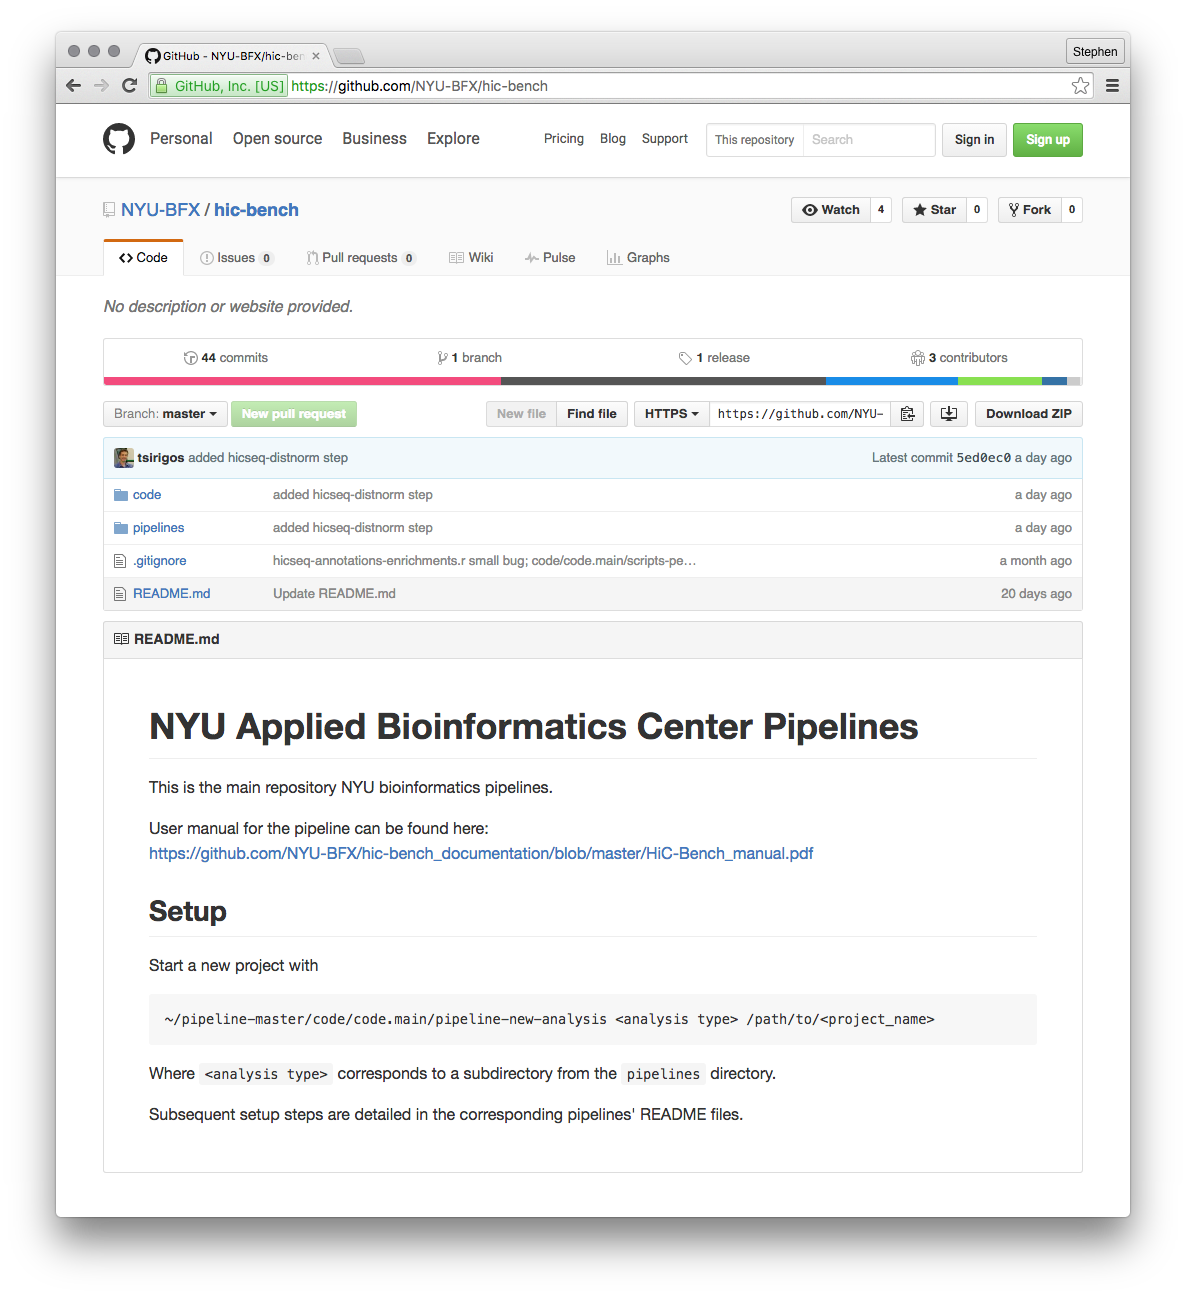
\includegraphics[width=1.0\linewidth]{./Figures/github_repo}
\caption{Our ChIP-Seq pipeline is part of the HiC-Bench software package, available on GitHub}
\label{fig:github_repo}
\end{figure}

%----------------------------------------------------------------------------------------
%	ACKNOWLEDGEMENTS
%----------------------------------------------------------------------------------------
\vspace{2.5cm}
\begin{beamerboxesrounded}{Future Developments}
\begin{itemize}
\item Automated motif analysis with HOMER and MEME-ChIP
\item Contaminant analysis
\item Peak enrichment analysis
\end{itemize}
\end{beamerboxesrounded}\hfill

\begin{beamerboxesrounded}{Acknowledgements}

This work used computing resources at the Laura and Isaac Perlmutter Cancer Center, which is supported by Cancer Center Support Grant P30CA016087.
A. Tsirigos was supported by a Research Scholar Grant, RSG-15-189-01-RMC
from the American Cancer Society. 
This work also used computing resources at the High Performance Computing Facility of the Center for Health Informatics and Bioinformatics at the NYU Langone Medical Center. \\

\end{beamerboxesrounded}\hfill
%----------------------------------------------------------------------------------------
%	SOFTWARE 
%----------------------------------------------------------------------------------------
\begin{beamerboxesrounded}{Software}
\begin{itemize}
\item \footnotesize{Web: \href{http://www.med.nyu.edu/ocs/applied-bioinformatics-center}{http://www.med.nyu.edu/ocs/applied-bioinformatics-center}}
\item \footnotesize{GitHub: \href{https://github.com/NYU-BFX/hic-bench}{https://github.com/NYU-BFX/hic-bench}}
\item \footnotesize{Zenodo: \href{https://zenodo.org/record/47676}{https://zenodo.org/record/47676}}
\item \footnotesize{Contact: \href{mailto:stephen.kelly@nyumc.org}{\textbf{stephen.kelly@nyumc.org}}, \href{mailto:aristotelis.tsirigos@nyumc.org}{\textbf{aristotelis.tsirigos@nyumc.org}}}
% \item \LaTeXe~ \fmtversion
\end{itemize}

\end{beamerboxesrounded}\hfill

% 3 % ~~~~~~~~~~~~~~~~~~~~~~~~~~~~~~ % ~~~~~~~~~~~~~~~~~~~~~~~~~~~
\end{column} % End of the third column

\end{columns} % End of all the columns in the poster

% FRAME % ~~~~~~~~~~~~~~~~~~~~~~~~~~~~~~ % ~~~~~~~~~~~~~~~~~~~~~~~~~~~
% ~~~~~~~~~~~~~~~~~~~~~~~~~~~~~~~~~~~~~~ % ~~~~~~~~~~~~~~~~~~~~~~~~~~~
\end{frame} % End of the enclosing frame

\end{document}
